\documentclass[tikz,border=10pt]{standalone}
\usetikzlibrary{calc}
\begin{document}
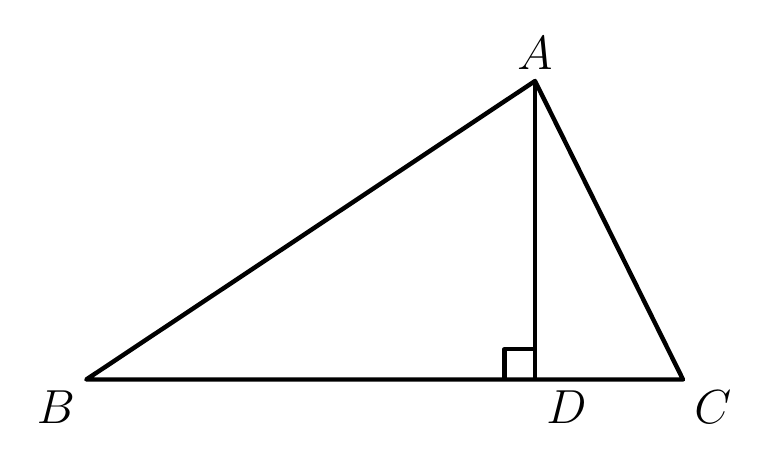
\begin{tikzpicture}[line width=1.6pt, line join=round]
% Coordinates: s = 0.020101 cm/px, origin at ink-bbox centre (236,159.5) px
\coordinate (A) at (1.9096,1.8915);
\coordinate (B) at (-3.7890,-1.8995);
\coordinate (C) at (3.7890,-1.8995);
\coordinate (D) at (1.9096,-1.8995);

% Triangle sides
\draw (A) -- (B) -- (C) -- cycle;

% Altitude AD (solid)
\draw (A) -- (D);

% Right-angle mark at D (toward B and up toward A), side about 0.387 cm
\draw (D)++(-0.3867,0) -- ++(0,0.3867) -- ++(0.3867,0);

% Labels
\node[above, font=\fontsize{16.5}{19.8}\selectfont] at (A) {$A$};
\node[below left, font=\fontsize{16.5}{19.8}\selectfont] at (B) {$B$};
\node[below right, font=\fontsize{16.5}{19.8}\selectfont] at (C) {$C$};
\node[below right, font=\fontsize{16.5}{19.8}\selectfont] at (D) {$D$};
\end{tikzpicture}
\end{document}